% Options for packages loaded elsewhere
% Options for packages loaded elsewhere
\PassOptionsToPackage{unicode}{hyperref}
\PassOptionsToPackage{hyphens}{url}
\PassOptionsToPackage{dvipsnames,svgnames,x11names}{xcolor}
%
\documentclass[
  letterpaper,
  DIV=11,
  numbers=noendperiod]{scrartcl}
\usepackage{xcolor}
\usepackage{amsmath,amssymb}
\setcounter{secnumdepth}{5}
\usepackage{iftex}
\ifPDFTeX
  \usepackage[T1]{fontenc}
  \usepackage[utf8]{inputenc}
  \usepackage{textcomp} % provide euro and other symbols
\else % if luatex or xetex
  \usepackage{unicode-math} % this also loads fontspec
  \defaultfontfeatures{Scale=MatchLowercase}
  \defaultfontfeatures[\rmfamily]{Ligatures=TeX,Scale=1}
\fi
\usepackage{lmodern}
\ifPDFTeX\else
  % xetex/luatex font selection
\fi
% Use upquote if available, for straight quotes in verbatim environments
\IfFileExists{upquote.sty}{\usepackage{upquote}}{}
\IfFileExists{microtype.sty}{% use microtype if available
  \usepackage[]{microtype}
  \UseMicrotypeSet[protrusion]{basicmath} % disable protrusion for tt fonts
}{}
\makeatletter
\@ifundefined{KOMAClassName}{% if non-KOMA class
  \IfFileExists{parskip.sty}{%
    \usepackage{parskip}
  }{% else
    \setlength{\parindent}{0pt}
    \setlength{\parskip}{6pt plus 2pt minus 1pt}}
}{% if KOMA class
  \KOMAoptions{parskip=half}}
\makeatother
% Make \paragraph and \subparagraph free-standing
\makeatletter
\ifx\paragraph\undefined\else
  \let\oldparagraph\paragraph
  \renewcommand{\paragraph}{
    \@ifstar
      \xxxParagraphStar
      \xxxParagraphNoStar
  }
  \newcommand{\xxxParagraphStar}[1]{\oldparagraph*{#1}\mbox{}}
  \newcommand{\xxxParagraphNoStar}[1]{\oldparagraph{#1}\mbox{}}
\fi
\ifx\subparagraph\undefined\else
  \let\oldsubparagraph\subparagraph
  \renewcommand{\subparagraph}{
    \@ifstar
      \xxxSubParagraphStar
      \xxxSubParagraphNoStar
  }
  \newcommand{\xxxSubParagraphStar}[1]{\oldsubparagraph*{#1}\mbox{}}
  \newcommand{\xxxSubParagraphNoStar}[1]{\oldsubparagraph{#1}\mbox{}}
\fi
\makeatother

\usepackage{color}
\usepackage{fancyvrb}
\newcommand{\VerbBar}{|}
\newcommand{\VERB}{\Verb[commandchars=\\\{\}]}
\DefineVerbatimEnvironment{Highlighting}{Verbatim}{commandchars=\\\{\}}
% Add ',fontsize=\small' for more characters per line
\usepackage{framed}
\definecolor{shadecolor}{RGB}{241,243,245}
\newenvironment{Shaded}{\begin{snugshade}}{\end{snugshade}}
\newcommand{\AlertTok}[1]{\textcolor[rgb]{0.68,0.00,0.00}{#1}}
\newcommand{\AnnotationTok}[1]{\textcolor[rgb]{0.37,0.37,0.37}{#1}}
\newcommand{\AttributeTok}[1]{\textcolor[rgb]{0.40,0.45,0.13}{#1}}
\newcommand{\BaseNTok}[1]{\textcolor[rgb]{0.68,0.00,0.00}{#1}}
\newcommand{\BuiltInTok}[1]{\textcolor[rgb]{0.00,0.23,0.31}{#1}}
\newcommand{\CharTok}[1]{\textcolor[rgb]{0.13,0.47,0.30}{#1}}
\newcommand{\CommentTok}[1]{\textcolor[rgb]{0.37,0.37,0.37}{#1}}
\newcommand{\CommentVarTok}[1]{\textcolor[rgb]{0.37,0.37,0.37}{\textit{#1}}}
\newcommand{\ConstantTok}[1]{\textcolor[rgb]{0.56,0.35,0.01}{#1}}
\newcommand{\ControlFlowTok}[1]{\textcolor[rgb]{0.00,0.23,0.31}{\textbf{#1}}}
\newcommand{\DataTypeTok}[1]{\textcolor[rgb]{0.68,0.00,0.00}{#1}}
\newcommand{\DecValTok}[1]{\textcolor[rgb]{0.68,0.00,0.00}{#1}}
\newcommand{\DocumentationTok}[1]{\textcolor[rgb]{0.37,0.37,0.37}{\textit{#1}}}
\newcommand{\ErrorTok}[1]{\textcolor[rgb]{0.68,0.00,0.00}{#1}}
\newcommand{\ExtensionTok}[1]{\textcolor[rgb]{0.00,0.23,0.31}{#1}}
\newcommand{\FloatTok}[1]{\textcolor[rgb]{0.68,0.00,0.00}{#1}}
\newcommand{\FunctionTok}[1]{\textcolor[rgb]{0.28,0.35,0.67}{#1}}
\newcommand{\ImportTok}[1]{\textcolor[rgb]{0.00,0.46,0.62}{#1}}
\newcommand{\InformationTok}[1]{\textcolor[rgb]{0.37,0.37,0.37}{#1}}
\newcommand{\KeywordTok}[1]{\textcolor[rgb]{0.00,0.23,0.31}{\textbf{#1}}}
\newcommand{\NormalTok}[1]{\textcolor[rgb]{0.00,0.23,0.31}{#1}}
\newcommand{\OperatorTok}[1]{\textcolor[rgb]{0.37,0.37,0.37}{#1}}
\newcommand{\OtherTok}[1]{\textcolor[rgb]{0.00,0.23,0.31}{#1}}
\newcommand{\PreprocessorTok}[1]{\textcolor[rgb]{0.68,0.00,0.00}{#1}}
\newcommand{\RegionMarkerTok}[1]{\textcolor[rgb]{0.00,0.23,0.31}{#1}}
\newcommand{\SpecialCharTok}[1]{\textcolor[rgb]{0.37,0.37,0.37}{#1}}
\newcommand{\SpecialStringTok}[1]{\textcolor[rgb]{0.13,0.47,0.30}{#1}}
\newcommand{\StringTok}[1]{\textcolor[rgb]{0.13,0.47,0.30}{#1}}
\newcommand{\VariableTok}[1]{\textcolor[rgb]{0.07,0.07,0.07}{#1}}
\newcommand{\VerbatimStringTok}[1]{\textcolor[rgb]{0.13,0.47,0.30}{#1}}
\newcommand{\WarningTok}[1]{\textcolor[rgb]{0.37,0.37,0.37}{\textit{#1}}}

\usepackage{longtable,booktabs,array}
\usepackage{calc} % for calculating minipage widths
% Correct order of tables after \paragraph or \subparagraph
\usepackage{etoolbox}
\makeatletter
\patchcmd\longtable{\par}{\if@noskipsec\mbox{}\fi\par}{}{}
\makeatother
% Allow footnotes in longtable head/foot
\IfFileExists{footnotehyper.sty}{\usepackage{footnotehyper}}{\usepackage{footnote}}
\makesavenoteenv{longtable}
\usepackage{graphicx}
\makeatletter
\newsavebox\pandoc@box
\newcommand*\pandocbounded[1]{% scales image to fit in text height/width
  \sbox\pandoc@box{#1}%
  \Gscale@div\@tempa{\textheight}{\dimexpr\ht\pandoc@box+\dp\pandoc@box\relax}%
  \Gscale@div\@tempb{\linewidth}{\wd\pandoc@box}%
  \ifdim\@tempb\p@<\@tempa\p@\let\@tempa\@tempb\fi% select the smaller of both
  \ifdim\@tempa\p@<\p@\scalebox{\@tempa}{\usebox\pandoc@box}%
  \else\usebox{\pandoc@box}%
  \fi%
}
% Set default figure placement to htbp
\def\fps@figure{htbp}
\makeatother





\setlength{\emergencystretch}{3em} % prevent overfull lines

\providecommand{\tightlist}{%
  \setlength{\itemsep}{0pt}\setlength{\parskip}{0pt}}



 


\KOMAoption{captions}{tableheading}
\makeatletter
\@ifpackageloaded{caption}{}{\usepackage{caption}}
\AtBeginDocument{%
\ifdefined\contentsname
  \renewcommand*\contentsname{Table of contents}
\else
  \newcommand\contentsname{Table of contents}
\fi
\ifdefined\listfigurename
  \renewcommand*\listfigurename{List of Figures}
\else
  \newcommand\listfigurename{List of Figures}
\fi
\ifdefined\listtablename
  \renewcommand*\listtablename{List of Tables}
\else
  \newcommand\listtablename{List of Tables}
\fi
\ifdefined\figurename
  \renewcommand*\figurename{Figure}
\else
  \newcommand\figurename{Figure}
\fi
\ifdefined\tablename
  \renewcommand*\tablename{Table}
\else
  \newcommand\tablename{Table}
\fi
}
\@ifpackageloaded{float}{}{\usepackage{float}}
\floatstyle{ruled}
\@ifundefined{c@chapter}{\newfloat{codelisting}{h}{lop}}{\newfloat{codelisting}{h}{lop}[chapter]}
\floatname{codelisting}{Listing}
\newcommand*\listoflistings{\listof{codelisting}{List of Listings}}
\makeatother
\makeatletter
\makeatother
\makeatletter
\@ifpackageloaded{caption}{}{\usepackage{caption}}
\@ifpackageloaded{subcaption}{}{\usepackage{subcaption}}
\makeatother
\usepackage{bookmark}
\IfFileExists{xurl.sty}{\usepackage{xurl}}{} % add URL line breaks if available
\urlstyle{same}
\hypersetup{
  pdftitle={Rapport de Projet: Pipeline OCR Intelligent},
  pdfauthor={Jean Luis Soto},
  colorlinks=true,
  linkcolor={blue},
  filecolor={Maroon},
  citecolor={Blue},
  urlcolor={Blue},
  pdfcreator={LaTeX via pandoc}}


\title{Rapport de Projet: Pipeline OCR Intelligent}
\usepackage{etoolbox}
\makeatletter
\providecommand{\subtitle}[1]{% add subtitle to \maketitle
  \apptocmd{\@title}{\par {\large #1 \par}}{}{}
}
\makeatother
\subtitle{Artefact School}
\author{Jean Luis Soto}
\date{2026-02-02}
\begin{document}
\maketitle

\renewcommand*\contentsname{Table of contents}
{
\hypersetup{linkcolor=}
\setcounter{tocdepth}{3}
\tableofcontents
}

\section{Compréhension du Métier (Business
Understanding)}\label{compruxe9hension-du-muxe9tier-business-understanding}

\subsection{Contexte du Projet}\label{contexte-du-projet}

Le commanditaire est une entreprise SaaS ERP spécialisée dans le secteur
douanier au Pérou, fournissant des services aux agents de fret, douanes,
opérateurs logistiques et importateurs/exportateurs.

Les utilisateurs interfacés avec le système doivent saisir de nombreuses
données techniques et commerciales sur les produits transitant par les
ports, conformément aux exigences strictes de la législation douanière
péruvienne. Actuellement, les entreprises doivent télécharger
manuellement sur le SaaS toutes les factures justifiant l'importation du
fret. Ce processus implique souvent le traitement de volumes importants
(d'une seule à des centaines de factures par interaction).

Ces factures servent de déclencheur critique pour l'exécution de divers
rapports réglementaires internes, tels que la détection de catégories de
produits importés, la somme des importations et le calcul des quantités.
Le processus manuel actuel est jugé \textbf{fastidieux, lent et sujet
aux erreurs humaines}.

\subsection{Problématique Actuelle}\label{probluxe9matique-actuelle}

L'organisation a précédemment tenté d'automatiser ce flux en
implémentant une solution OCR basée sur un outil de Deep Learning
(Google Document AI). Bien que les résultats des tests initiaux
(\texttt{proof\ of\ concept}) fussent prometteurs, la mise en production
a révélé des défaillances majeures:

\begin{itemize}
\item
  \textbf{Sur-apprentissage (Overfitting)} : Le modèle ne généralisait
  pas bien aux nouvelles factures ou aux variations mineures
  (off-setting).
\item
  \textbf{Coût de maintenance prohibitif} : Nécessité de ré-entraîner le
  modèle pour chaque nouveau client intégrant la plateforme. Ce
  processus de ré-entraînement prenait jusqu'à une demi-journée par
  client, sans garantie de succès pour le client suivant.
\end{itemize}

\subsection{Objectifs du Projet (Business
Objectives)}\label{objectifs-du-projet-business-objectives}

Face à ces échecs, les objectifs du nouveau projet sont clairs :

\begin{enumerate}
\def\labelenumi{\arabic{enumi}.}
\item
  \textbf{Automatisation Robuste} : Disposer d'une solution capable de
  lire les factures de manière automatisée sans nécessiter de
  ré-entraînement constant.
\item
  \textbf{Haute Précision} : Garantir une fiabilité élevée dans
  l'extraction des données critiques.
\item
  \textbf{Réduction des Coûts} : Obtenir des coûts opérationnels
  inférieurs à ceux de l'outil Document AI actuel.
\item
  \textbf{Performance (SLA)} : Respecter un niveau de service strict :
  \textbf{traiter 50 factures en moins de 5 minutes}, quel que soit le
  nombre de pages.
\item
  \textbf{Polyvalence} : Gérer efficacement l'hétérogénéité des formats
  et des langues.
\end{enumerate}

\subsection{Situation Technique}\label{situation-technique}

La solution doit être déployée sur \textbf{Google Cloud Platform (GCP)}
et être conçue pour être escalable. Le projet dispose actuellement d'un
jeu de données de vérité terrain (Ground Truth) de taille petite à
moyenne pour valider la nouvelle approche.

\section{Compréhension des Données (Data
Understanding)}\label{compruxe9hension-des-donnuxe9es-data-understanding}

\subsection{Nature des Données}\label{nature-des-donnuxe9es}

Les documents d'entrée sont exclusivement des fichiers PDF. Cependant,
leur origine varie grandement :

\begin{itemize}
\tightlist
\item
  Documents natifs numériques.
\item
  Documents numérisés (scans) ou photographiés.
\item
  \textbf{Hétérogénéité} : Une grande diversité de mises en page
  (layouts) et de langues, reflétant la nature internationale du
  commerce logistique.
\end{itemize}

\subsection{Structure des Données
Cibles}\label{structure-des-donnuxe9es-cibles}

Le modèle doit extraire les informations structurées selon un schéma
JSON précis, aligné avec les besoins de l'ERP douanier. Voici un exemple
de la structure attendue :

\begin{longtable}[]{@{}
  >{\raggedright\arraybackslash}p{(\linewidth - 2\tabcolsep) * \real{0.5000}}
  >{\raggedright\arraybackslash}p{(\linewidth - 2\tabcolsep) * \real{0.5000}}@{}}
\toprule\noalign{}
\begin{minipage}[b]{\linewidth}\raggedright
Champ
\end{minipage} & \begin{minipage}[b]{\linewidth}\raggedright
Description
\end{minipage} \\
\midrule\noalign{}
\endhead
\bottomrule\noalign{}
\endlastfoot
\texttt{supplier\_name} & Nom de l'entité émettrice de la facture. \\
\texttt{invoice\_id} & Identifiant unique du document. \\
\texttt{invoice\_date} & Date d'émission de la facture. \\
\texttt{currency} & Devise utilisée pour la transaction. \\
\texttt{total\_amount} & Montant total à payer. \\
\texttt{line\_items} & Liste des articles ou services facturés
(description, quantité, prix). \\
\end{longtable}

\begin{figure}[H]

{\centering 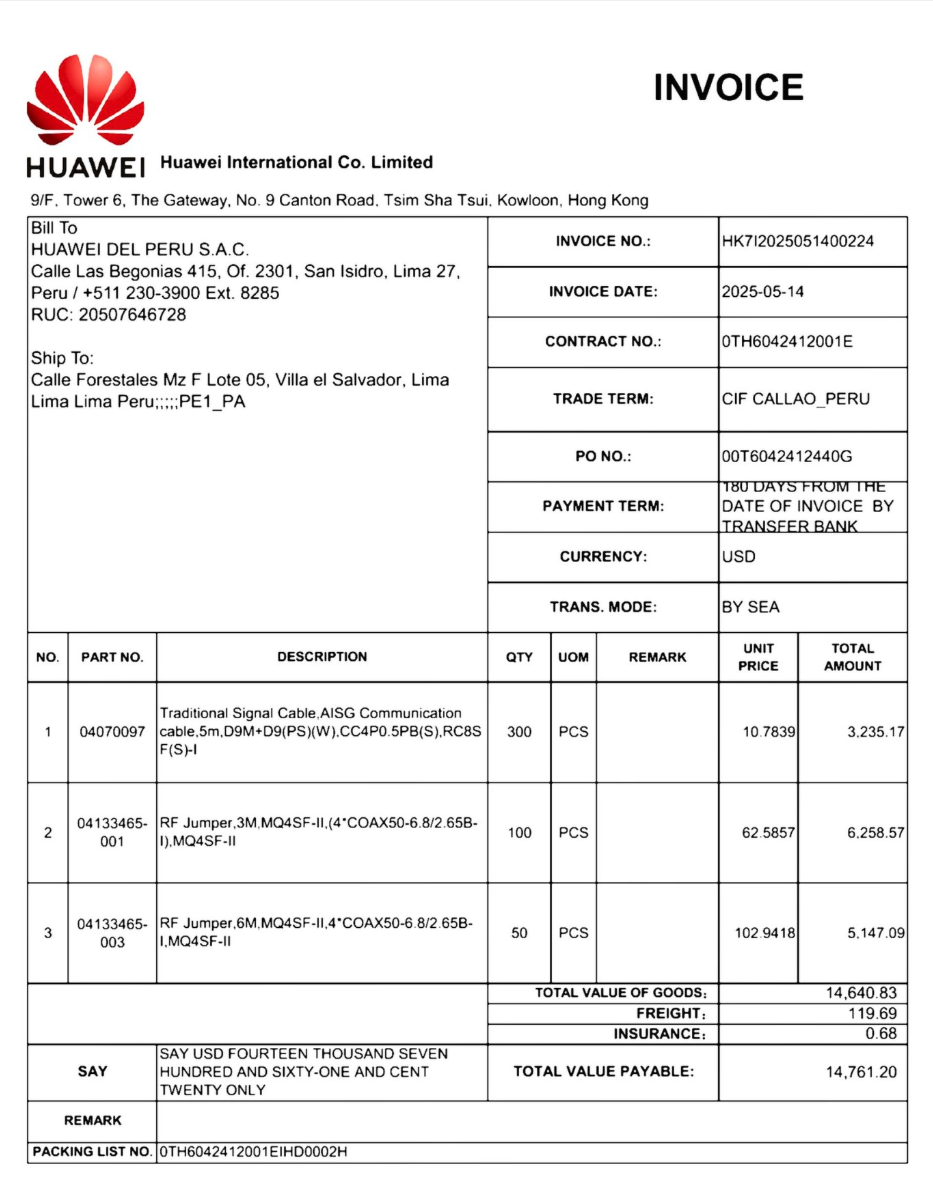
\includegraphics[width=0.5\linewidth,height=\textheight,keepaspectratio]{images/image_facture.png}

}

\caption{Facture example}

\end{figure}%

\begin{Shaded}
\begin{Highlighting}[]
\FunctionTok{\{}
  \DataTypeTok{"supplier\_name"}\FunctionTok{:} \StringTok{"Huawei International Co. Limited"}\FunctionTok{,} 
  \DataTypeTok{"invoice\_id"}\FunctionTok{:} \StringTok{"HK7l2025051400224"}\FunctionTok{,} 
  \DataTypeTok{"invoice\_date"}\FunctionTok{:} \StringTok{"2025{-}05{-}14"}\FunctionTok{,}
  \DataTypeTok{"line\_items"}\FunctionTok{:} \OtherTok{[}
    \FunctionTok{\{}
      \DataTypeTok{"description"}\FunctionTok{:} \StringTok{"Traditional Signal Cable, AISG Communication cable, 5m..."}\FunctionTok{,} 
      \DataTypeTok{"quantity"}\FunctionTok{:} \StringTok{"300"}\FunctionTok{,} 
      \DataTypeTok{"amount"}\FunctionTok{:} \StringTok{"3,235.17"}
    \FunctionTok{\}}\OtherTok{,} 
    \FunctionTok{\{}
      \DataTypeTok{"description"}\FunctionTok{:} \StringTok{"RF Jumper, 3M, MQ4SF{-}II, (4*COAX50{-}6.8/2.65B{-}I)..."}\FunctionTok{,} 
      \DataTypeTok{"quantity"}\FunctionTok{:} \StringTok{"100"}\FunctionTok{,} 
      \DataTypeTok{"amount"}\FunctionTok{:} \StringTok{"6,258.57"}
    \FunctionTok{\}}
  \OtherTok{]}
\FunctionTok{\}}
\end{Highlighting}
\end{Shaded}

\section{Préparation des Données (Data
Preparation)}\label{pruxe9paration-des-donnuxe9es-data-preparation}

\subsection{Ground Truth}\label{ground-truth}

La constitution du jeu de données de référence (\emph{Ground Truth}) a
représenté l'un des défis majeurs du projet. Initialement, les modèles
ont montré des performances insatisfaisantes en raison de plusieurs
incohérences critiques identifiées dans les données d'origine :

\begin{itemize}
\tightlist
\item
  \textbf{Diversité des formats de date} : Présence de formats très
  hétérogènes (dates écrites en toutes lettres, formats numériques
  variés), ce qui a complexifié la phase de validation automatique.
\item
  \textbf{Incomplétude et fragmentation des articles} : Certains
  articles présentaient des descriptions sur une ligne et des prix sur
  une autre, ou encore plusieurs descriptions fragmentées pour un même
  produit.
\item
  \textbf{Défis de standardisation} : Face à ces obstacles, une étape de
  standardisation rigoureuse a été nécessaire pour établir une base de
  données d'exemple cohérente.
\end{itemize}

Des efforts sont actuellement poursuivis pour affiner ce corpus afin de
garantir un niveau de fiabilité optimal pour les phases d'entraînement
et d'évaluation.

Voici un exemple du format JSON standardisé ciblé :

\begin{Shaded}
\begin{Highlighting}[]
\FunctionTok{\{}
  \DataTypeTok{"line\_items"}\FunctionTok{:} \OtherTok{[}
    \FunctionTok{\{}
      \DataTypeTok{"description"}\FunctionTok{:} \StringTok{"Câble de communication AISG"}\FunctionTok{,}
      \DataTypeTok{"quantity"}\FunctionTok{:} \StringTok{"300"}\FunctionTok{,}
      \DataTypeTok{"amount"}\FunctionTok{:} \KeywordTok{null} 
    \FunctionTok{\}}\OtherTok{,}
    \FunctionTok{\{}
      \DataTypeTok{"description"}\FunctionTok{:} \KeywordTok{null}\FunctionTok{,}
      \DataTypeTok{"quantity"}\FunctionTok{:} \KeywordTok{null}\FunctionTok{,}
      \DataTypeTok{"amount"}\FunctionTok{:} \StringTok{"3,235.17"}
    \FunctionTok{\}}
  \OtherTok{]}
\FunctionTok{\}}
\end{Highlighting}
\end{Shaded}

\subsection{État actuel du Pipeline de
Données}\label{uxe9tat-actuel-du-pipeline-de-donnuxe9es}

Actuellement, aucune étape automatisée de nettoyage ou de prétraitement
des fichiers PDF entrants n'a été mise en place en amont. Les documents
sont stockés en l'état, ce qui constitue un obstacle pour les modèles
d'IA, car la qualité visuelle brute d'un scan impacte directement le
taux de succès de l'OCR.

\subsection{Fondamentaux du Nettoyage
d'Images}\label{fondamentaux-du-nettoyage-dimages}

Pour pallier ce manque, une couche de traitement d'image robuste basée
sur \textbf{OpenCV} et \textbf{Pillow} a été introduite. Voici l'analyse
détaillée des algorithmes implémentés et de leur justification technique
:

\begin{itemize}
\tightlist
\item
  \textbf{Upscaling Intelligent} :

  \begin{itemize}
  \tightlist
  \item
    \emph{Problème} : Certains scans arrivent en basse résolution (72
    DPI), rendant les petits caractères illisibles pour l'OCR.
  \item
    \emph{Solution} : Si la largeur de l'image est inférieure à 2000px,
    un redimensionnement avec l'algorithme de rééchantillonnage de
    Lanczos (\texttt{resize\_if\_small}) est appliqué, ce qui préserve
    mieux les détails des bords que l'interpolation bicubique standard.
  \end{itemize}
\item
  \textbf{Denoising} :

  \begin{itemize}
  \tightlist
  \item
    \emph{Problème} : Le ``bruit poivre et sel'' classique des scanners
    anciens crée des artefacts noirs isolés.
  \item
    \emph{Solution} : Application d'un \texttt{MedianFilter}.
    Contrairement au flou gaussien qui ``bave'' les contours, le filtre
    médian élimine le bruit ponctuel tout en gardant les arêtes des
    lettres nettes.
  \end{itemize}
\item
  \textbf{Deskewing} :

  \begin{itemize}
  \tightlist
  \item
    \emph{Problème} : Une facture scannée avec une rotation de 3° suffit
    à chasser le texte hors des colonnes attendues pour l'extraction de
    tableaux.
  \item
    \emph{Solution} : Détection de l'angle d'inclinaison via
    \texttt{cv2.minAreaRect} sur un masque binaire
    (\texttt{THRESH\_OTSU}), suivie d'une rotation inverse.
  \end{itemize}
\item
  \textbf{CLAHE} :

  \begin{itemize}
  \tightlist
  \item
    \emph{Problème} : L'égalisation d'histogramme classique ``brûle''
    les zones claires. Sur une photo de facture avec des ombres (ex:
    prise avec un smartphone), le contraste n'est pas uniforme.
  \item
    \emph{Solution} : CLAHE améliore le contraste \emph{localement} sur
    des tuiles (8x8 pixels), permettant de révéler du texte caché dans
    l'ombre sans surexposer le reste du document.
  \end{itemize}
\item
  \textbf{Ajustements Colorimétriques} :

  \begin{itemize}
  \tightlist
  \item
    Optimisation fine utilisant \texttt{ImageEnhance} pour maximiser le
    ``Pop'' du texte noir sur fond blanc, guidée par les hyperparamètres
    trouvés via Optuna.
  \end{itemize}
\end{itemize}

\subsection{Stratégies de Prétraitement
Implémentées}\label{stratuxe9gies-de-pruxe9traitement-impluxe9mentuxe9es}

\subsubsection{Approche ML Traditionnelle (Optimisation
Scientifique)}\label{approche-ml-traditionnelle-optimisation-scientifique}

Plutôt que de définir ces paramètres de nettoyage arbitrairement (``au
feeling''), une méthodologie rigoureuse d'optimisation bayésienne des
hyperparamètres (HPO) a été adoptée en utilisant le framework
\textbf{Optuna}.

Le pipeline exécute de multiples itérations (``trials'') en faisant
varier les paramètres pour maximiser une métrique objective : le
\textbf{F1-Score} global de l'extraction.

\begin{itemize}
\tightlist
\item
  \textbf{Paramètres optimisés} :

  \begin{itemize}
  \tightlist
  \item
    Facteur de contraste (Range: 1.0 - 1.8)
  \item
    Facteur de luminosité (Range: 1.0 - 1.4)
  \item
    Taille du noyau de débruitage (Denoise Kernel: 1, 3, 5)
  \item
    Activation conditionnelle du CLAHE et du Deskewing (Booléen)
  \end{itemize}
\end{itemize}

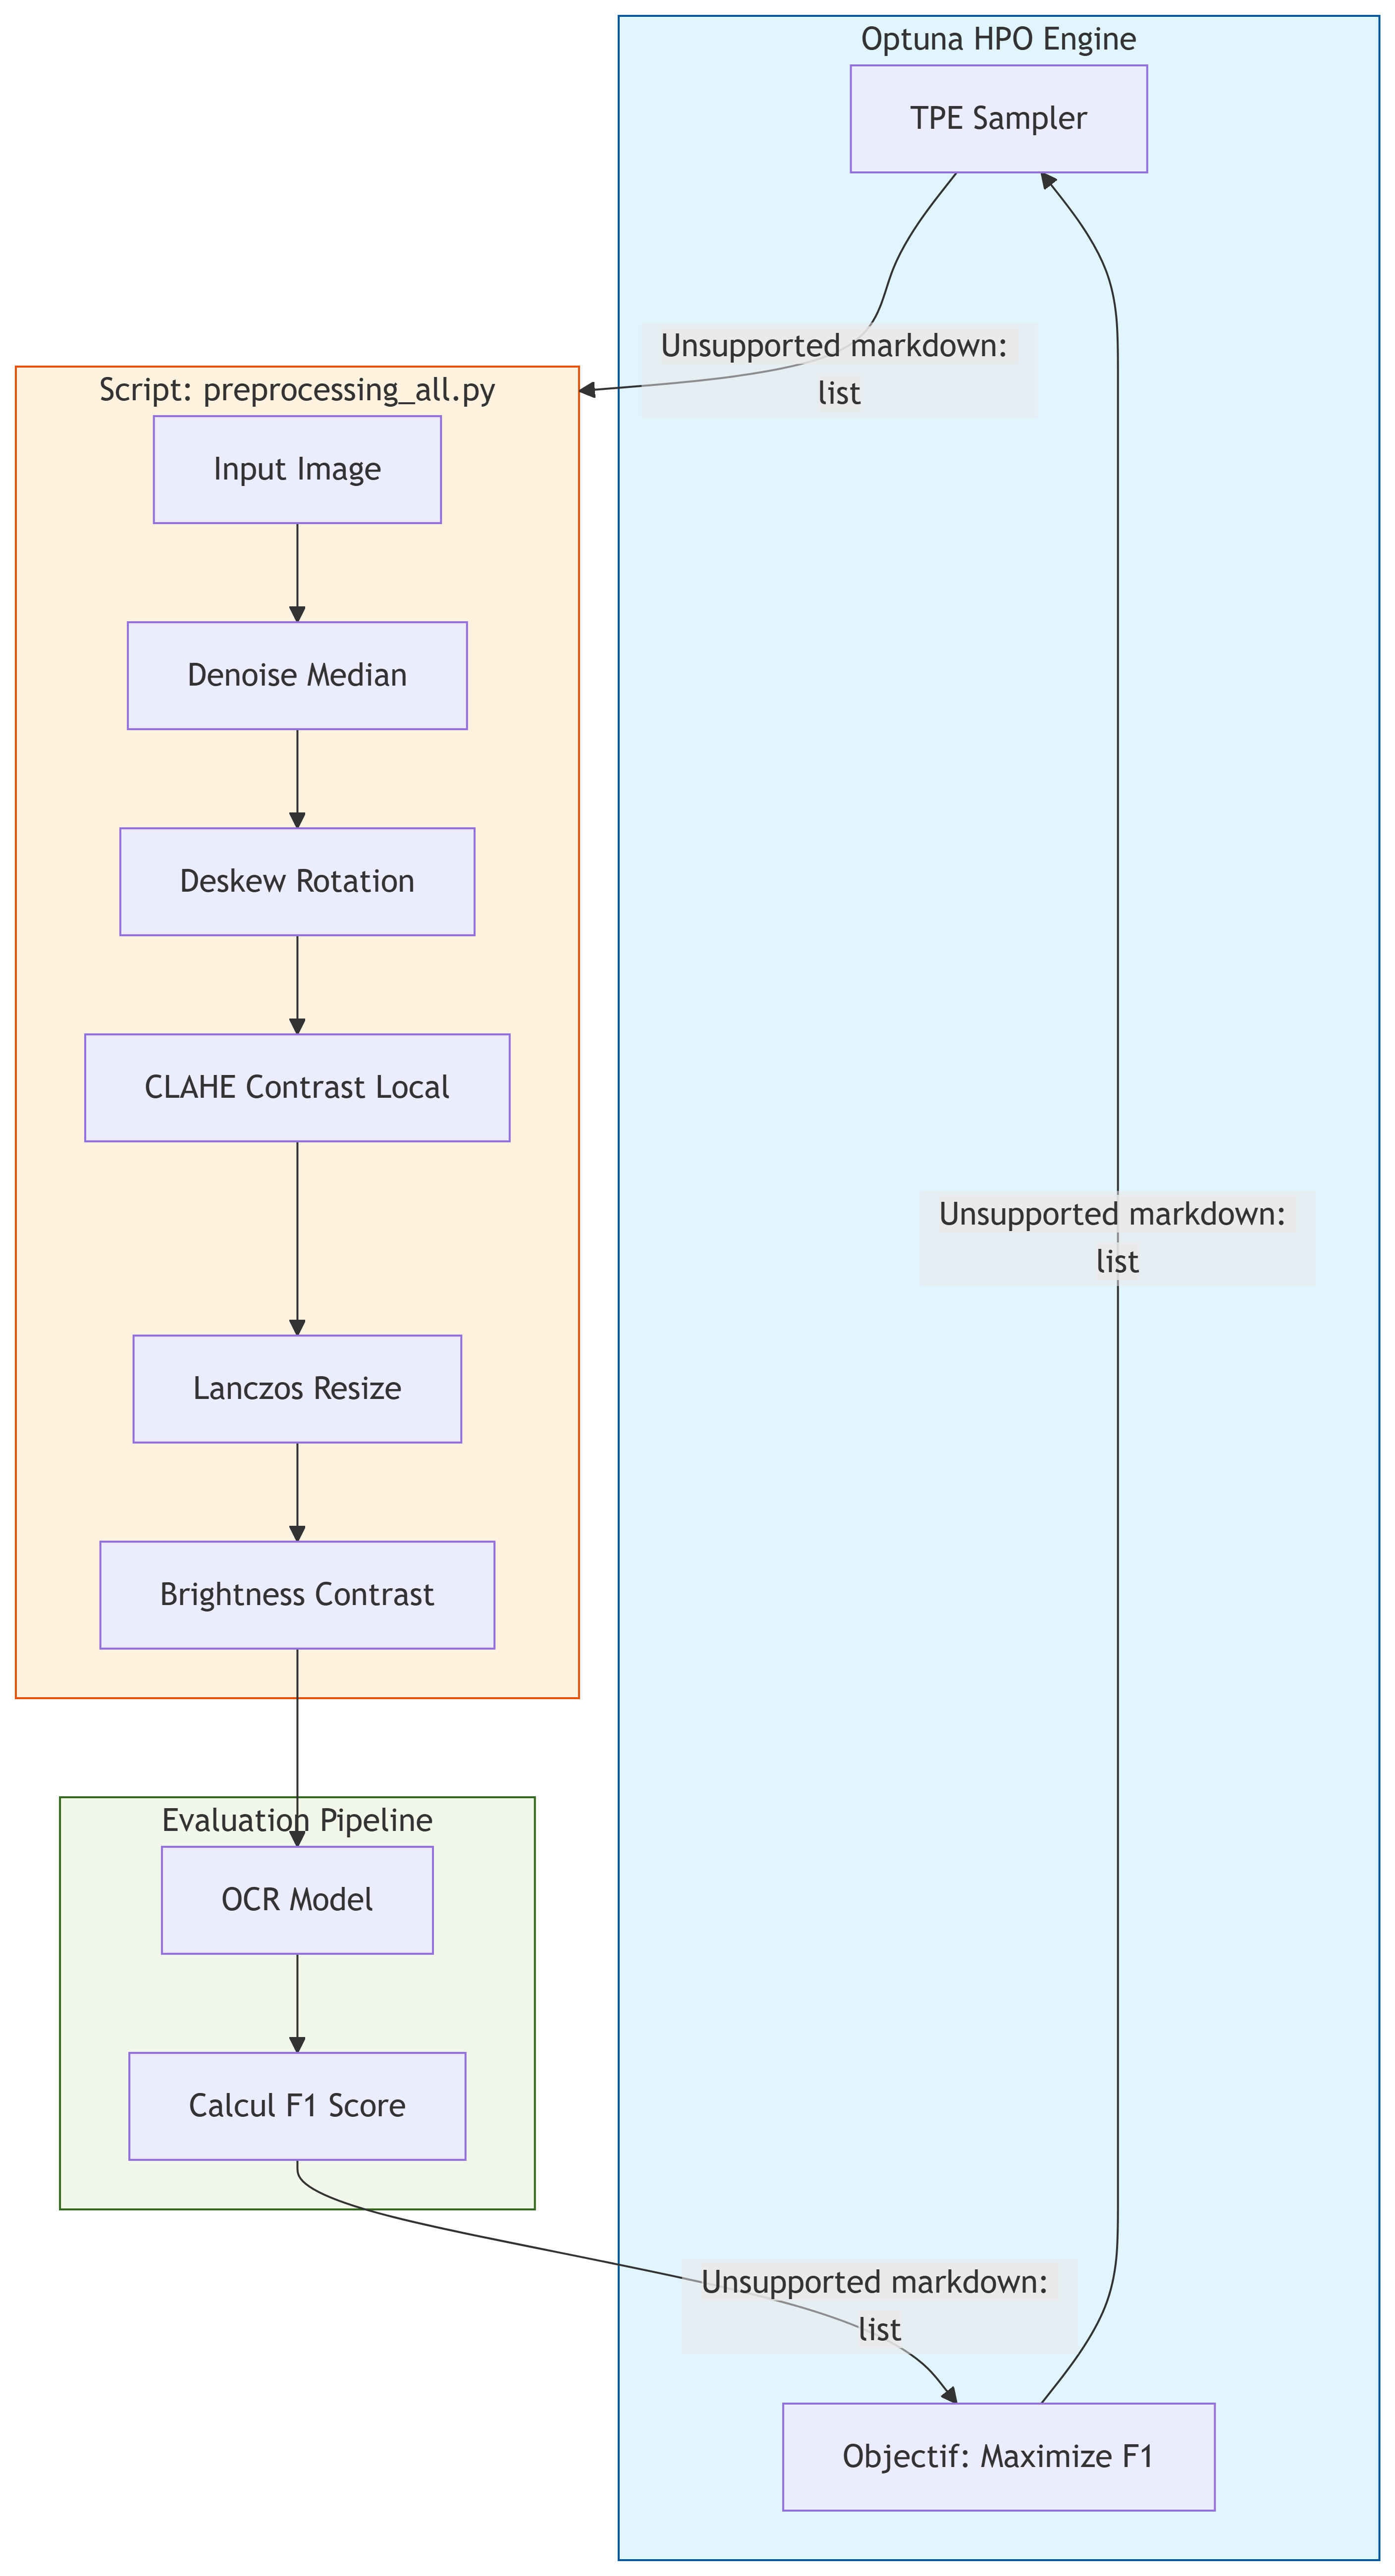
\includegraphics[width=7.33in,height=13.54in]{index_files/figure-latex/mermaid-figure-1.png}

Cette approche transforme la configuration du pré-traitement d'un art
subjectif en une science mesurable, garantissant que chaque filtre
appliqué contribue statistiquement à la qualité du résultat final.

\subsubsection{Prémices d'un Agent IA de
Prétraitement}\label{pruxe9mices-dun-agent-ia-de-pruxe9traitement}

Pour résoudre le manque de flexibilité de l'approche statique (qui
applique les mêmes paramètres agnostiques à tous les documents), les
bases de ce qui deviendra un \textbf{Agent IA de Prétraitement} ont été
posées.

L'idée est de créer un système capable d'\textbf{évaluer d'abord la
qualité visuelle} spécifique du document (luminosité, flou, biais) avant
de décider dynamiquement des actions à entreprendre.

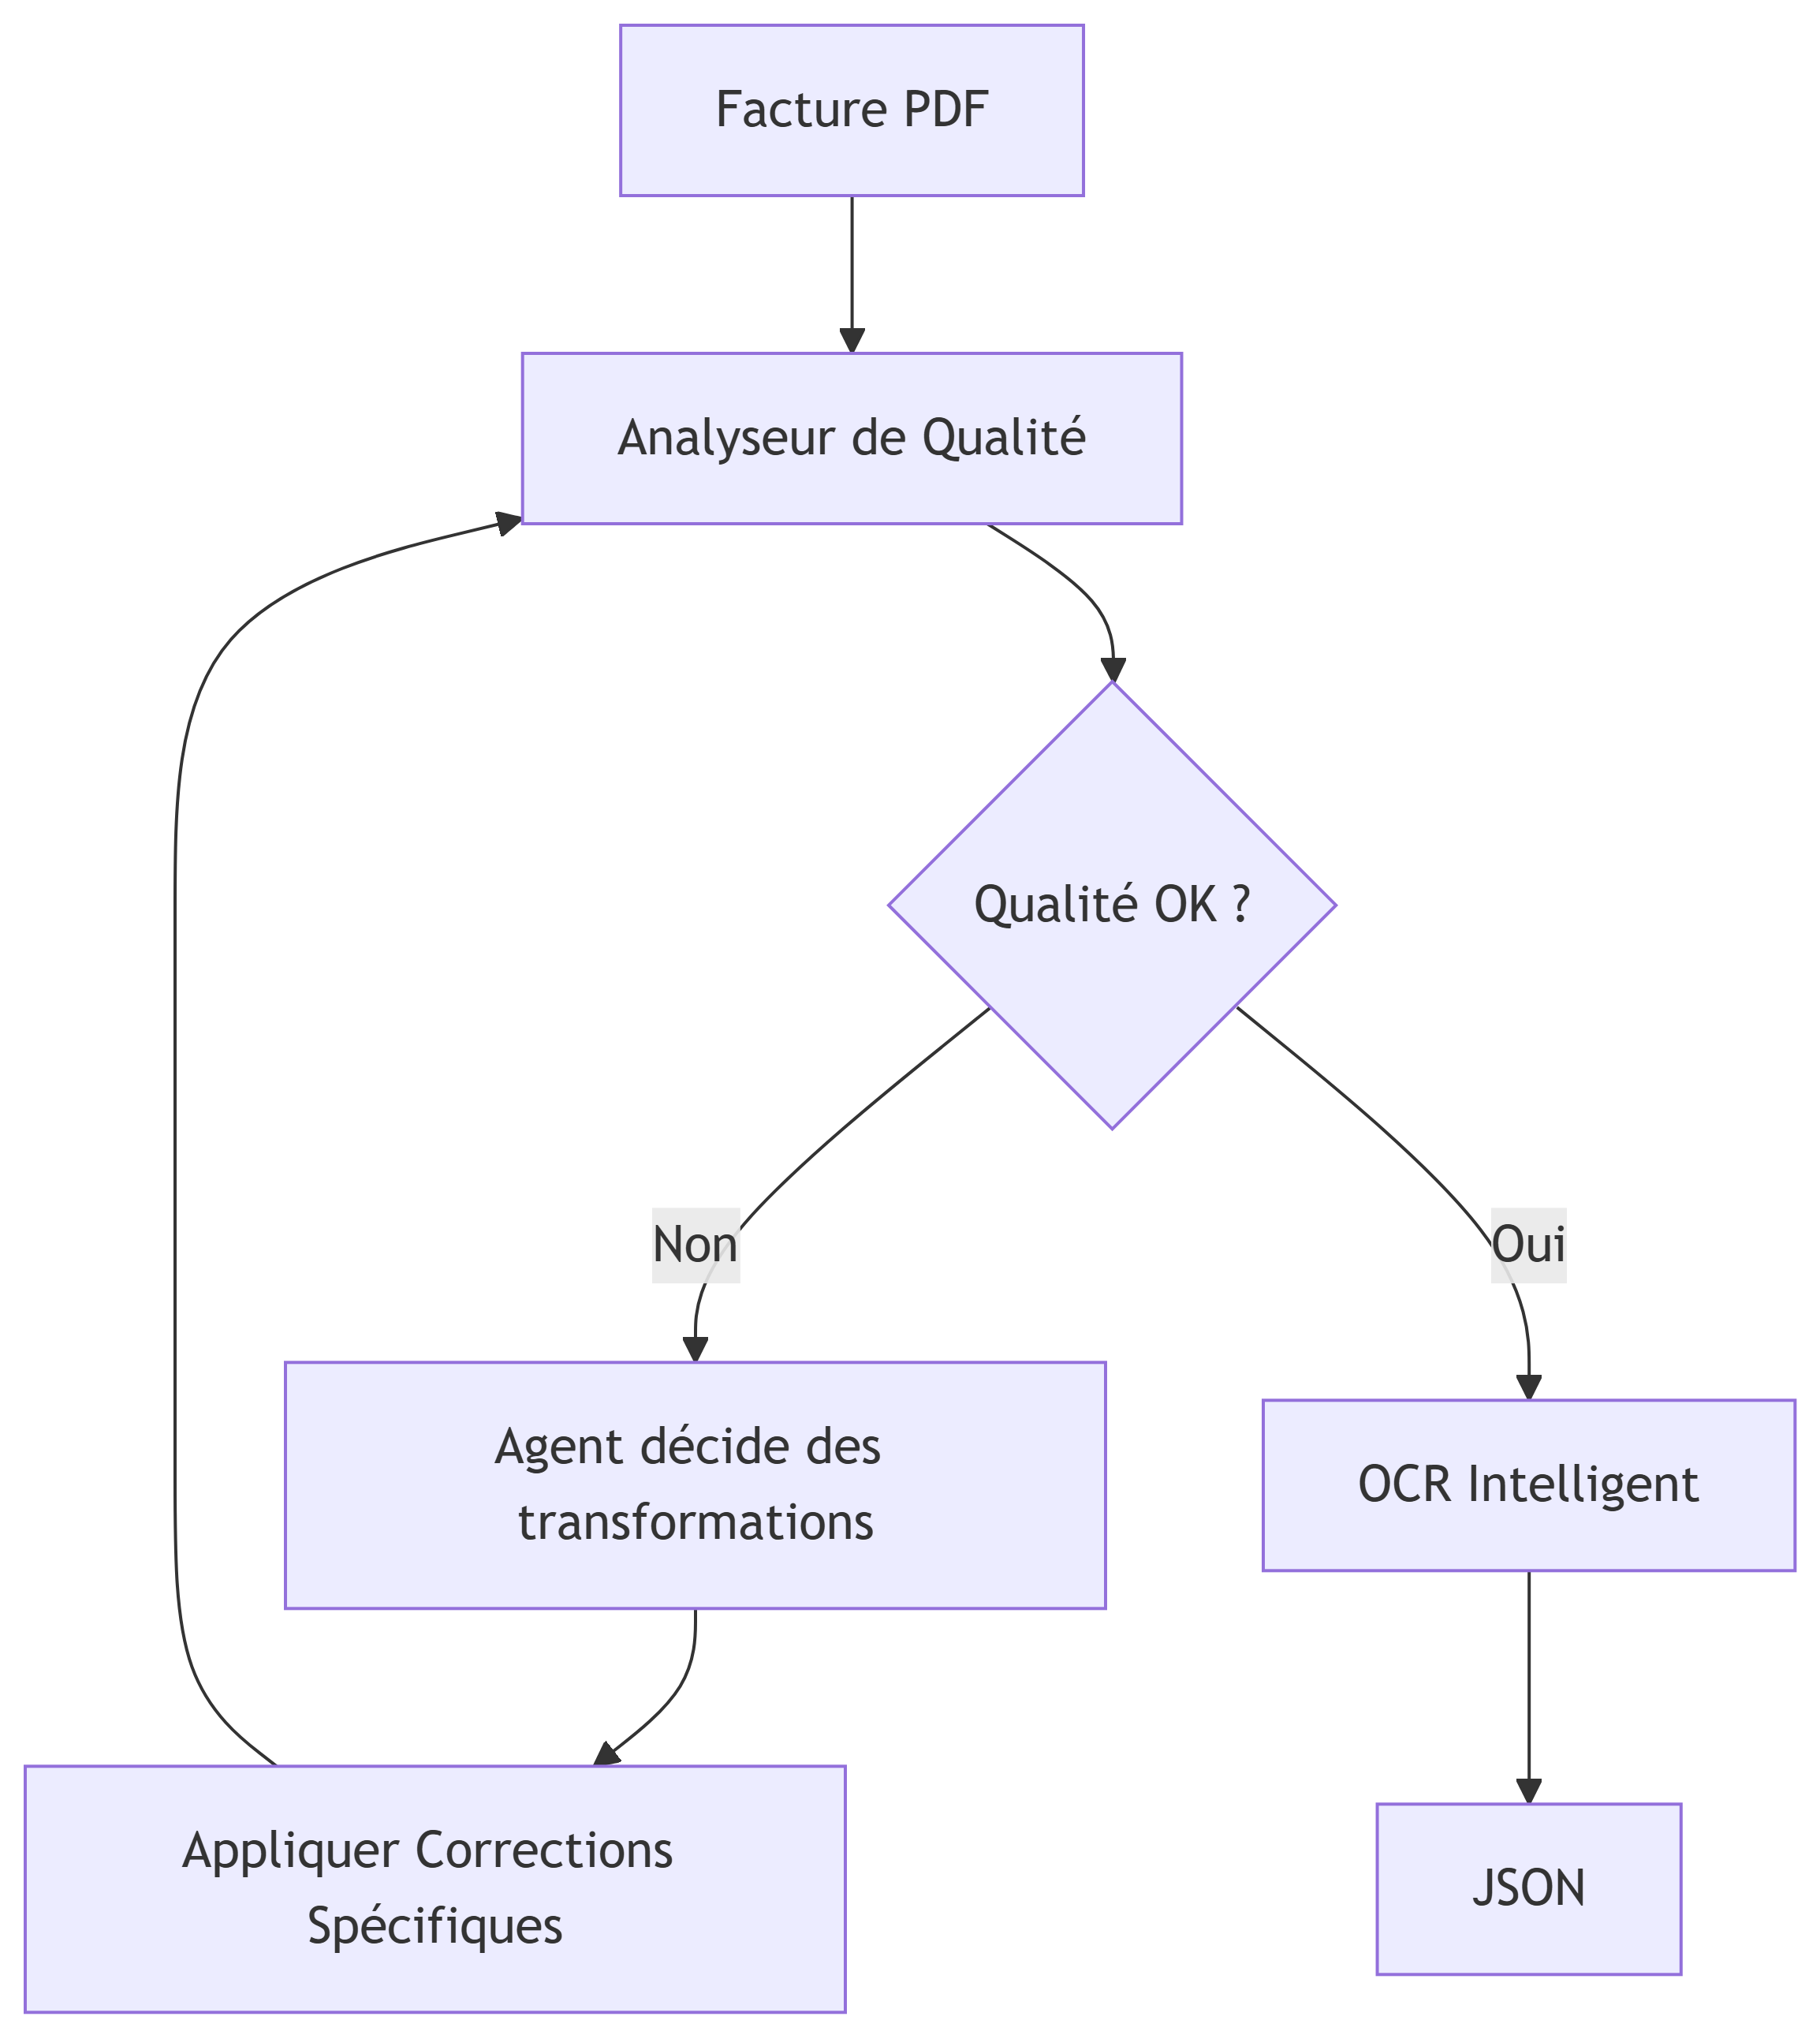
\includegraphics[width=6.01in,height=6.73in]{index_files/figure-latex/mermaid-figure-3.png}

La logique repose sur une boucle de feedback intelligente : tant que le
score de qualité visuelle n'est pas optimal, l'agent itère sur les
paramètres. Cela permet de traiter une photo sombre différemment d'un
scan clair, là où l'approche traditionnelle échouerait sur l'un des
deux.

\section{Modélisation (Modeling)}\label{moduxe9lisation-modeling}

\subsection{Architecture du Pipeline}\label{architecture-du-pipeline}

Le projet repose sur une architecture modulaire :

\begin{enumerate}
\def\labelenumi{\arabic{enumi}.}
\tightlist
\item
  \textbf{Ingestion}: Chargement depuis Google Cloud Storage (GCS).
\item
  \textbf{Preprocessing}: OpenCV / Python.
\item
  \textbf{Extraction (Modèles IA)} : voir section suivante.
\end{enumerate}

\subsection{Analyse Comparative des Modèles
OCR}\label{analyse-comparative-des-moduxe8les-ocr}

Pour ce projet, plusieurs familles de modèles ont été évaluées afin de
trouver l'équilibre optimal entre précision, coût et maintenabilité.

\subsubsection{1. Typologie des Modèles}\label{typologie-des-moduxe8les}

Deux catégories principales sont distinguées :

\begin{itemize}
\tightlist
\item
  \textbf{OCR Traditionnel (ex: Tesseract)} :

  \begin{itemize}
  \tightlist
  \item
    \emph{Principe} : Analyse géométrique pixel par pixel pour
    identifier des caractères.
  \item
    \emph{Avantages} : Gratuit, extrêmement rapide, s'exécute 100\% en
    local (confidentialité totale), mature.
  \item
    \emph{Limites} : ``Aveugle'' au contexte sémantique. Il peut lire
    ``O'' au lieu de ``0'' sans comprendre qu'il s'agit d'un prix.
    Nécessite souvent des expressions régulières (Regex) complexes pour
    structurer la donnée \emph{a posteriori}.
  \end{itemize}
\item
  \textbf{LLM Vision / Extracteurs (ex: Mistral, Llama, Gemini)} :

  \begin{itemize}
  \tightlist
  \item
    \emph{Principe} : Modèles de langage géants capables de ``voir''
    (via un encodeur visuel ou un OCR intermédiaire) et de
    ``comprendre'' le document globalement.
  \item
    \emph{Avantages} : Compréhension sémantique forte. Capacité à
    corriger une faute de frappe (``Totla'' -\textgreater{} ``Total'')
    grâce au contexte. Sortie directe en JSON structuré prêt à l'emploi.
  \item
    \emph{Limites} : Coût d'inférence (API), latence plus élevée, risque
    d'hallucination (inventer une donnée manquante).
  \end{itemize}
\end{itemize}

\subsubsection{2. Modèles Sélectionnés et
Benchmarks}\label{moduxe8les-suxe9lectionnuxe9s-et-benchmarks}

Trois modèles spécifiques ont été sélectionnés pour l'implémentation
finale, excluant Google Document AI (propriétaire et ``boîte noire'')
pour privilégier le contrôle et la flexibilité.

\begin{longtable}[]{@{}
  >{\raggedright\arraybackslash}p{(\linewidth - 10\tabcolsep) * \real{0.1667}}
  >{\raggedright\arraybackslash}p{(\linewidth - 10\tabcolsep) * \real{0.1667}}
  >{\raggedright\arraybackslash}p{(\linewidth - 10\tabcolsep) * \real{0.1667}}
  >{\raggedright\arraybackslash}p{(\linewidth - 10\tabcolsep) * \real{0.1667}}
  >{\raggedright\arraybackslash}p{(\linewidth - 10\tabcolsep) * \real{0.1667}}
  >{\raggedright\arraybackslash}p{(\linewidth - 10\tabcolsep) * \real{0.1667}}@{}}
\toprule\noalign{}
\begin{minipage}[b]{\linewidth}\raggedright
Modèle
\end{minipage} & \begin{minipage}[b]{\linewidth}\raggedright
Type
\end{minipage} & \begin{minipage}[b]{\linewidth}\raggedright
Licence
\end{minipage} & \begin{minipage}[b]{\linewidth}\raggedright
Coût estimé / 1k pages
\end{minipage} & \begin{minipage}[b]{\linewidth}\raggedright
Vitesse
\end{minipage} & \begin{minipage}[b]{\linewidth}\raggedright
Précision Contextuelle
\end{minipage} \\
\midrule\noalign{}
\endhead
\bottomrule\noalign{}
\endlastfoot
\textbf{Tesseract 5} & OCR Classique & Open Source (Apache 2.0) &
\textbf{0.00 €} (CPU) & \textbf{Très Rapide} (\textless1s) & Faible
(Nécessite Regex) \\
\textbf{Llama 3 (via Groq)} & LLM (Text-to-JSON) & Open Weights & Très
Faible & Ultra Rapide (LPU) & \textbf{Excellente} \\
\textbf{Mistral 7B / Large} & LLM (Génératif) & Open Weights / API &
Faible / Moyen & Moyenne & Très Bonne \\
\end{longtable}

\subsubsection{3. Justification du Choix
Final}\label{justification-du-choix-final}

\begin{itemize}
\tightlist
\item
  \textbf{Tesseract} a été conservé comme \textbf{Baseline} (référence
  de base). Il permet de valider si l'ajout d'une IA complexe apporte
  réellement de la valeur par rapport à une solution gratuite.
\item
  \textbf{Mistral} a été choisi pour sa robustesse en multilingue et sa
  facilité d'utilisation.
\item
  \textbf{Llama 3} (implémenté via l'accélérateur Groq) a démontré une
  capacité exceptionnelle à respecter le SLA de 5 minutes pour 50
  factures grâce à son inférence ultra-rapide.
\end{itemize}

\subsection{Pipeline d'Inférence (Architecture
End-to-End)}\label{pipeline-dinfuxe9rence-architecture-end-to-end}

L'architecture globale de la solution est conçue pour être modulaire et
scalable sur GCP, intégrant des techniques d'ingénierie logicielle
avancées pour maximiser la performance.

\subsubsection{Workflow Complet}\label{workflow-complet}

Le flux de données suit ces étapes clés : 1. \textbf{Ingestion
Asynchrone} : Récupération parallèle des PDF depuis le Bucket GCS via
\texttt{asyncio}. 2. \textbf{Pré-traitement (3 Modes)} : * \emph{None} :
Image brute. * \emph{Standard} : Application de filtres basiques. *
\emph{Intelligent (Optuna)} : Paramètres optimisés dynamiquement. 3.
\textbf{Inférence (Batch)} : Envoi optimisé des requêtes aux modèles
(Mistral API, Groq) avec gestion de la concurrence pour minimiser la
latence réseau. 4. \textbf{Post-traitement et Validation} : Parsing,
nettoyage Regex (pour Tesseract), et validation stricte du schéma JSON
via Pydantic. 5. \textbf{Output} : Stockage persistant des résultats
validés.

\subsubsection{Optimisation de la Performance
(SLA)}\label{optimisation-de-la-performance-sla}

Pour atteindre l'objectif de \textbf{50 factures en \textless{} 5
minutes}, les mesures suivantes ont été implémentées : *
\textbf{Concurrence Asynchrone} : Utilisation intensive de
\texttt{Python\ asyncio} pour non-bloquer les I/O (lectures GCS, appels
API). * \textbf{Parallélisme CPU} : Utilisation de
\texttt{ProcessPoolExecutor} pour distribuer la charge lourde du
traitement d'image (OpenCV) sur tous les cœurs disponibles.

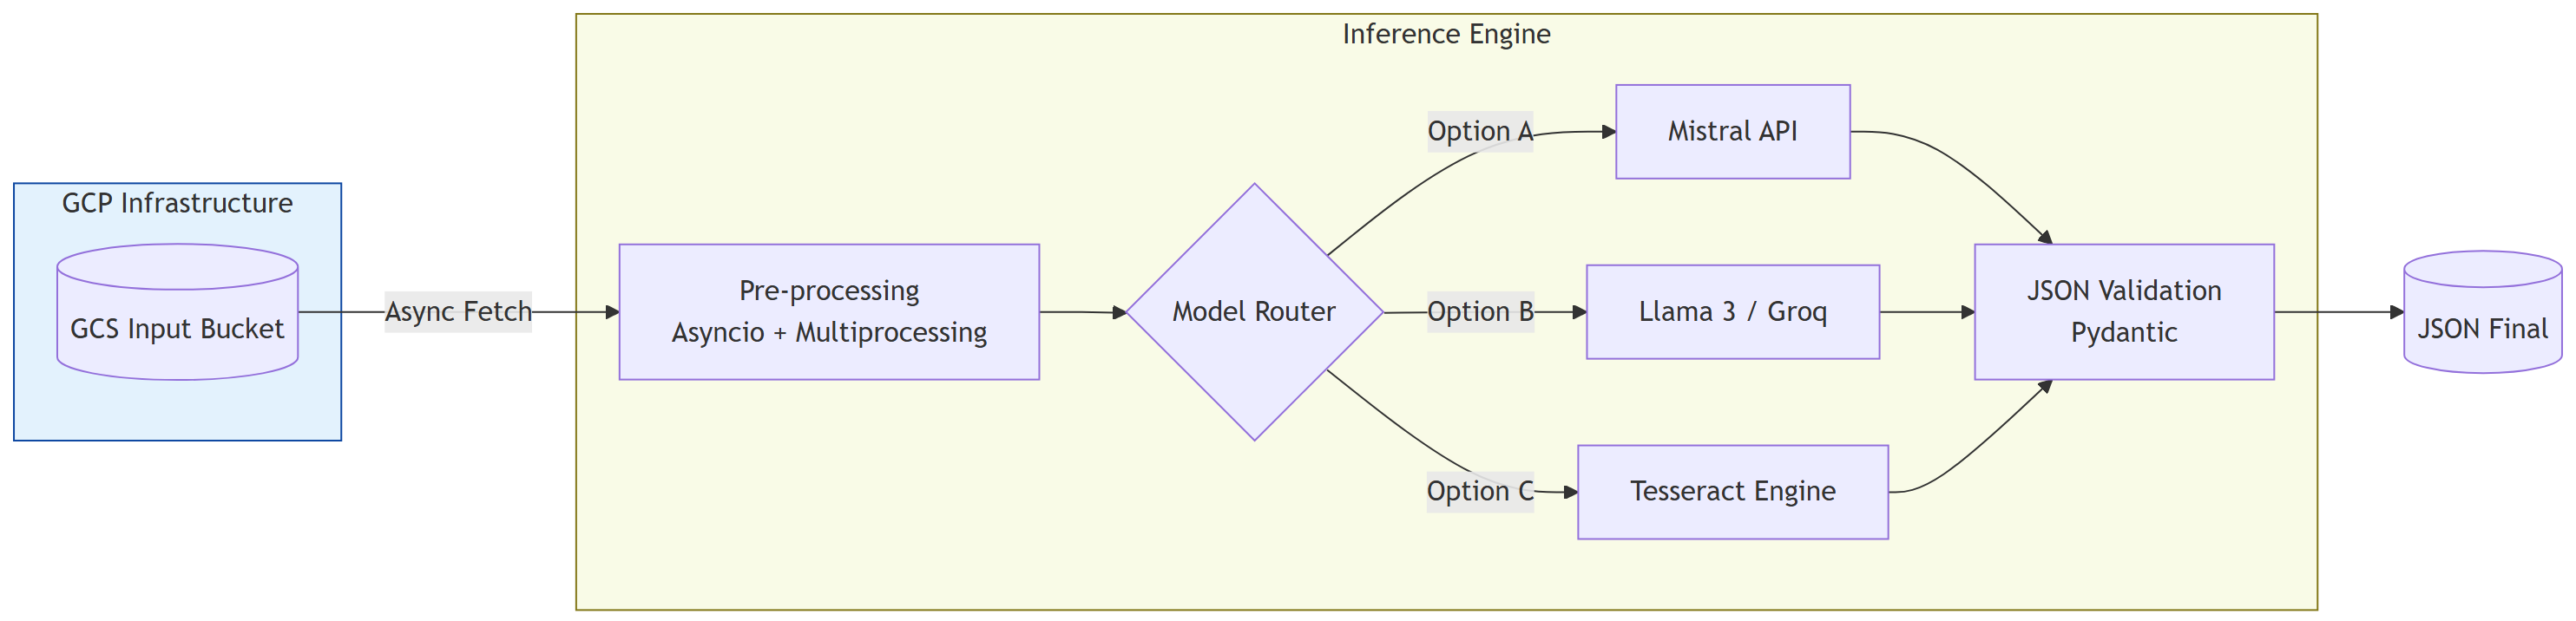
\includegraphics[width=15.47in,height=3.75in]{index_files/figure-latex/mermaid-figure-2.png}

\subsection{Configuration des
Services}\label{configuration-des-services}

La configuration est centralisée dans des fichiers \texttt{.env} et
gérée par \texttt{pydantic} pour valider les schémas d'entrée/sortie.

\section{Évaluation (Evaluation)}\label{uxe9valuation-evaluation}

\subsection{Méthodologie}\label{muxe9thodologie}

L'évaluation repose sur MLflow pour le tracking des expériences. Les
métriques clés sont : * \textbf{Exact Match Rate (EMR)} pour les champs
d'en-tête. * \textbf{F1 Score} pour les lignes produits (tolérance floue
via \texttt{RapidFuzz}). * \textbf{Character Error Rate (CER)} pour
mesurer la qualité de la transcription textuelle.

\subsection{Résultats du Benchmark}\label{ruxe9sultats-du-benchmark}

\emph{(Insérer ici les graphiques générés par MLflow ou des tableaux de
résultats)}

\begin{quote}
Le modèle \textbf{{[}MODELE\_GAGNANT{]}} a obtenu les meilleures
performances avec un F1-Score global de \textbf{XX\%}.
\end{quote}

\section{Déploiement (Deployment)}\label{duxe9ploiement-deployment}

\subsection{API REST (C9)}\label{api-rest-c9}

Le modèle sélectionné a été encapsulé dans une API REST développée avec
\textbf{FastAPI}. * Endpoint: \texttt{POST\ /extract} * Entrée: Fichier
PDF/Image * Sortie: JSON structuré

\begin{Shaded}
\begin{Highlighting}[]
\AttributeTok{@app.post}\NormalTok{(}\StringTok{"/extract"}\NormalTok{)}
\ControlFlowTok{async} \KeywordTok{def}\NormalTok{ extract\_invoice(}\BuiltInTok{file}\NormalTok{: UploadFile):}
    \CommentTok{\# Logique d\textquotesingle{}appel du modèle}
    \ControlFlowTok{return}\NormalTok{ \{}\StringTok{"data"}\NormalTok{: extracted\_json\}}
\end{Highlighting}
\end{Shaded}

\subsection{Application Utilisateur}\label{application-utilisateur}

Une interface \textbf{Streamlit} permet aux utilisateurs finaux de : 1.
Uploader une facture. 2. Visualiser les résultats extraits en temps
réel. 3. Corriger les erreurs éventuelles (Human-in-the-loop).

\subsection{Industrialisation}\label{industrialisation}

\begin{itemize}
\tightlist
\item
  \textbf{Containerisation}: Utilisation de Docker pour packager
  l'application.
\item
  \textbf{CI/CD}: Pipeline de déploiement (théorique ou implémenté via
  GitHub Actions).
\item
  \textbf{Monitoring}: Suivi de la dérive du modèle via MLflow.
\end{itemize}

\section{Conclusion}\label{conclusion}

Ce projet a permis de valider l'ensemble des compétences du référentiel
RNCP37827BC02, du choix technologique jusqu'au déploiement d'une
solution d'IA opérationnelle et monitorée.




\end{document}
